\chapter{Models}\label{ch:models}

This chapter presents an in-depth exploration of various models used in the automatic generation of 3D models. It bridges the theoretical foundations laid in the previous chapters with practical applications and technologies that are developing the field of 3D modeling. Furthermore, it delves into different categories of model generation, specifically focusing on 3D models generated from text and images. This comprehensive analysis not only highlights the diversity and complexity of current methods but also underscores the rapid advancements and potential future developments in this domain. The below timeline shows the chronological development of these models, offering a perspective on how the field has progressed over time.

\begin{figure}[H]
    \centering
      \includegraphics[width=\textwidth]{figures/timelineMethods.png}
      \caption{Timeline of generative 3D modeling technologies: This figure outlines important milestones in the development of the key methods discussed in this thesis.}~\label{fig:timelineMethods}
\end{figure}

The chapter is structured to critically examine the methodologies, strengths, and limitations of each model. This detailed exploration provides an in-depth understanding of the current state of 3D model generation, emphasizing both the technological intricacies and their practical implications.

\section{3D from Text input}
\label{3d from text}
//TODO

\subsection{Dreamfields}
\label{dreamfields}

The concept proposed by \citeauthor{jainDreamFields} was groundbreaking, as they introduced the innovative approach of training a 2D diffusion model on images to learn 3D structure. This approach eliminated the reliance on pre-existing 3D Models, which is often scarce in large datasets.
\subsection{Dreamfusion}\label{dreamfusion}

DreamFusion leverages Neural Radiance Fields (NeRFs) \citep{mildenhallNERF} and uses a novel technique called Score Distillation Sampling (SDS) \citep{pooleDreamfusion} which "generates high-fidelity coherent 3D objects and scenes for a diverse set of user-provided text prompts \citep{pooleDreamfusion}. However, it is important to note that for the practical purposes of this thesis, \emph{Stable} DreamFusion \citep{stable-dreamfusion}, is used,  which is an open-source variant of DreamFusion. This variant introduces some differences compared to the original model. Stable DreamFusion modifies the original Imagen model by incorporating Stable Diffusion \citep{rombachStableDiffusion}, a latent diffusion model. It also employs the "multi-resolution grid encoder [from torch-ngp] to implement the NeRF backbone" \citep{stable-dreamfusion} and uses the Adan optimizer as the default option \citep{stable-dreamfusion}.

DreamFusion, a product of Google Research, embodies a significant leap in the domain of text-to-3D synthesis, a realm where textual descriptions are converted into three-dimensional visual models. It builds upon recent advancements in text-to-image synthesis driven by diffusion models trained on extensive image-text datasets. Unlike its predecessors, DreamFusion adeptly navigates the challenges posed by the lack of large-scale datasets of labeled 3D assets and efficient architectures for denoising 3D data. 

The genesis of DreamFusion lies in the evolution of Dream Fields, a generative 3D AI system unveiled by Google in late 2021. Dream Fields initially married OpenAI's image analysis model, CLIP, with Neural Radiance Fields (NeRF) to foster the generation of 3D views from text. DreamFusion further refined this approach by introducing a new loss based on Google's large AI image model, Imagen, thus paving the way for enhanced text to 3D synthesis.


At the core of DreamFusion's operation lies a fusion of Google's Imagen and NeRF's 3D capabilities. Imagen, a pre-trained 2D text-image diffusion model, forms the basis for text to 3D synthesis in DreamFusion. This synergy with NeRF, specialized for 3D generation tasks, enables the recovery and synthesis of new views of a particular scene from unobserved angles. DreamFusion employs a novel method termed Score Distillation Sampling (SDS) to optimize a 3D scene given a text caption. SDS allows for the generation of samples from a diffusion model by optimizing a loss function. This method demonstrates the versatility of pre-trained image diffusion models as priors, enabling the optimization of samples in an arbitrary parameter space such as a 3D space, provided there is a mapping back mechanism. Understanding the underlying principles of Neural Radiance Fields (NeRF), Score Distillation Sampling (SDS), and the functionality of the Imagen model is crucial for a comprehensive grasp of DreamFusion's architecture. The primary application of DreamFusion is the generation of 3D models from textual descriptions. This capability has vast potential across various fields including, but not limited to, virtual reality, gaming, and educational domains where interactive 3D models can enhance user engagement and learning experiences. 

Moreover, DreamFusion's ability to create relightable 3D objects and merge multiple 3D models into one scene opens avenues for more complex applications, enabling the creation of intricate, text-driven 3D scenes and animations.



Benefits:
- **Data Efficiency**: DreamFusion circumvents the need for large-scale 3D labeled datasets, which are often a bottleneck in 3D synthesis projects.
- **Generative Capability**: The generation of high-quality, relightable 3D objects based on textual input extends the boundaries of generative models.

Limitations:
- **Model Maturity**: The generated 3D models, although promising, may not yet attain a high level of accuracy, indicating a scope for further refinement.
- **Computational Resources**: The processing power required for the generation of 3D models could be substantial, posing challenges for resource-constrained environments.


DreamFusion marks a significant stride in bridging textual descriptions with 3D visualization using artificial intelligence. Its innovative architecture, built upon the synergy between Google's Imagen and NeRF, alongside the introduction of Score Distillation Sampling, lays a solid foundation for future advancements in text-to-3D synthesis. While the journey towards perfecting this technology continues, the potential applications and benefits of DreamFusion are vast and poised to have a lasting impact on the fields of computer vision and artificial intelligence.


Score Distillation Sampling (SDS) is a technique introduced in DreamFusion to generate samples from a diffusion model by optimizing a loss function, allowing for the optimization of samples in an arbitrary parameter space, such as a 3D space. The core idea is to leverage the structure of diffusion models to enable tractable sampling via optimization. This is achieved by optimizing over parameters \( \theta \) such that \( \mathbf{x} = g(\theta) \) appears as a sample from the frozen diffusion model. A differentiable loss function is employed where plausible images incur a low loss, and implausible images incur a high loss.

Mathematically, the process can be broken down into several steps:

1. **Loss Function Optimization**:
    - The objective is to minimize a diffusion training loss with respect to a generated datapoint \( \mathbf{x} = g(\theta) \), expressed as:
     \[ \theta^{*} = \text{arg min}_{\theta} \mathcal{L}_{\text{Diff}}(\phi, \mathbf{x} = g(\theta)) \]
   
    - In this step, DreamFusion tries to find the best set of parameters (denoted by \( \theta \)) that would generate a 3D model from text. It does this by minimizing a "loss function," which is a way to measure how far off the generated model is from what is desired. The goal is to adjust the parameters \( \theta \) so that this loss is as small as possible.

2. **Gradient Computation**:
   - The gradient of \( \mathcal{L}_{\text{Diff}} \) is given by:
     \[ \nabla_{\theta}\mathcal{L}_{\text{Diff}}(\phi,\mathbf{x}=g(\theta))=\mathbb{E}_{t,\epsilon}\Bigg[w(t)\left(\hat{\epsilon}_{\phi}({\mathbf{z}}_{t};y,t)-\epsilon\right)\frac{\partial\hat{\epsilon}_{\phi}({\mathbf{z}}_{t};y,t)}{\mathbf{z}_t}\frac{\partial\mathbf{x}}{\partial\theta}\Bigg] \]
   - Here, \( w(t) \) is a weighting term, \( \hat{\epsilon}_{\phi}({\mathbf{z}}_{t};y,t) \) is the predicted noise, \( \epsilon \) is the true noise, and \( \frac{\partial\hat{\epsilon}_{\phi}({\mathbf{z}}_{t};y,t)}{\mathbf{z}_t} \) and \( \frac{\partial\mathbf{x}}{\partial\theta} \) are Jacobian terms. 

   - To minimize the loss, DreamFusion needs to know in which direction to adjust the parameters \( \theta \). This is done by computing the gradient, which tells us the direction in which the loss function is increasing. By moving the parameters in the opposite direction, the loss can be decreased. In the formula, the terms involving \( \hat{\epsilon}_{\phi} \) and \( \epsilon \) are comparing the predicted noise to the actual noise in the model, which helps in understanding how to adjust the parameters to get a better model.

3. **Effective Gradient**:
   - To bypass the computation of certain Jacobian terms, an effective gradient is proposed:
     \[ \nabla_{\theta}\mathcal{L}_{\text{SDS}}(\phi,\mathbf{x}=g(\theta))\triangleq\mathbb{E}_{t,\epsilon}\left[w(t)\left(\hat{\epsilon}_{\phi}({\mathbf{z}}_{t};y,t)-\epsilon\right){\partial\mathbf{x}\frac\partial\theta}\right] \]

    - The original gradient computation can be quite complex and computationally expensive. So, an alternative, simplified version of the gradient is used to make the optimization process more manageable. This simplified gradient still gives a good direction to adjust the parameters \( \theta \) to minimize the loss, but without some of the computational overhead of the original gradient computation.


In practice, the diffusion model predicts the update direction, obviating the need to backpropagate through the diffusion model. Hence, the model acts like an efficient, frozen critic that predicts image-space edits.

When compared to a method like Collaborative Score Distillation (CSD), it's noted that while SDS optimizes a single 3D representation to maintain a high likelihood as evaluated by the diffusion model, CSD tends to excel in capturing coherent geometry and allows for the learning of finer details. Moreover, CSD can produce diverse, high-quality samples without requiring changes in random seeds, indicating some of the areas where SDS might have room for improvement.

\begin{figure}[ht]
  \centering
    \includegraphics[width=1\columnwidth]{figures/Dreamfusion.png}
    \caption{Summatized functionality of Dreamfusion}\label{fig:figureDreamfusion}
  \end{figure}
\subsection{Point-E}
\label{point-e}

Point-E operates through a two-stage generation process, resulting in point clouds. The initial stage involves the creation of an image using the text-to-image model GLIDE \citep{nicholGLIDE}, which was "fine tuned on 3D renderings" \citep{nicholPointE}. In the next stage, known as the image-to-3D model, RGB point-clouds are created with a stack of diffusion models \citep{nicholPointE}.
\subsection{Shap-E}
\label{shap-e}

Shap-E involves training an encoder which "produces a latent representation of a 3D asset" \citep{junShapeE}. In a second step, a diffusion prior on the obtained latent representations is trained, conditioning it on images or text descriptions to capture additional information \citep{junShapeE}.

\section{3D from Image}\label{3d from image}

The conversion of two-dimensional images into three-dimensional models represents a significant challenge in the domain of computer vision and 3D modeling. This section explores the methodologies and technologies employed in transforming 2D images into 3D models, a process that has profound implications in various fields, including virtual reality, gaming, and medical imaging. Techniques such as Magic 123 and Wonder3D will be thoroughly analyzed.

\subsection{Magic 123}
\label{Magic123}

//TODO

\begin{figure}[ht]
    \centering
      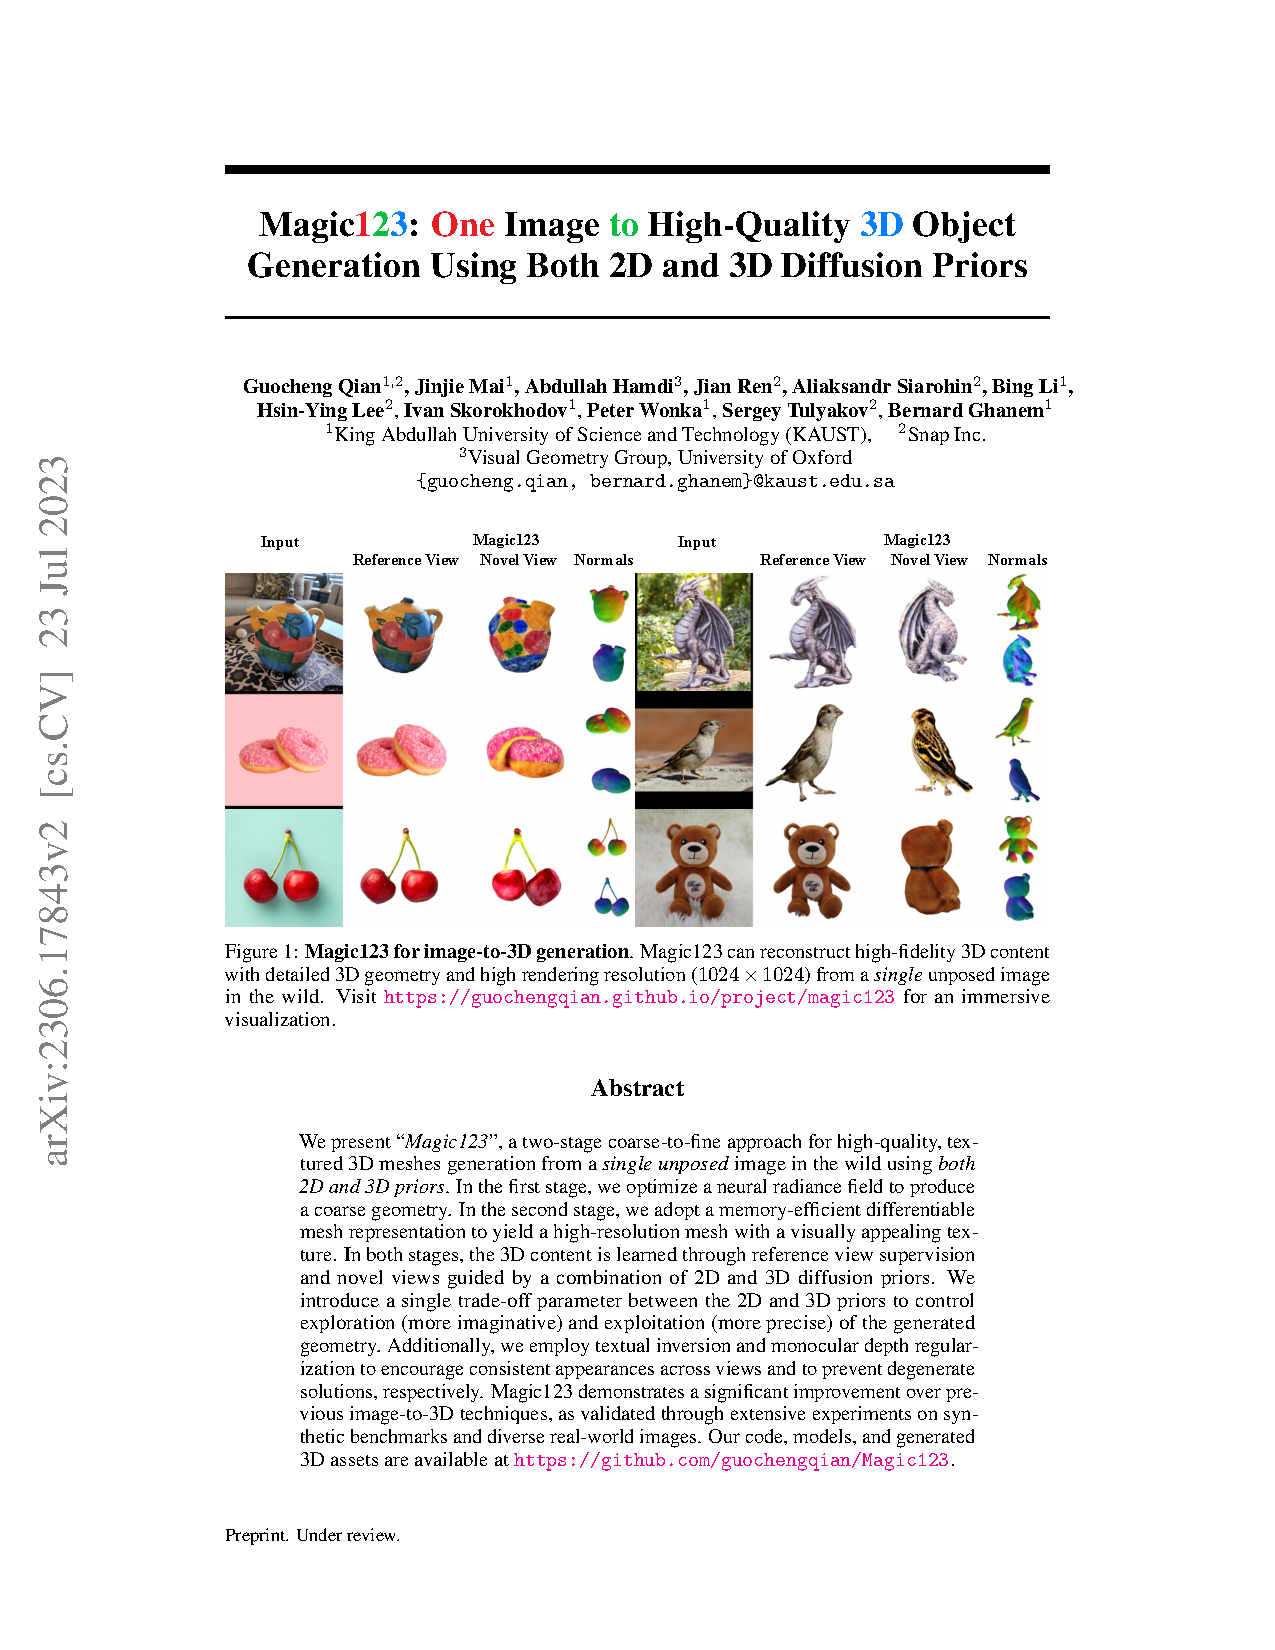
\includegraphics[width=1\columnwidth]{figures/Magic123.png}
      \caption{Summatized functionality of Magic123}\label{fig:figureMagic123}
\end{figure}
\subsection{Wonder 3D}\label{Wonder3D}

\citeauthor{long2023wonder3d} introduce Wonder3D, a technique that stands apart  from its predecessors primarily through its adeptness in generating not just color images, but also consistent multi-view normal maps. This method leverages a cross-domain diffusion model, ``extends the stable diffusion framework to model the joint distribution of two different domains, i.e., normals and colors'' \citep{long2023wonder3d}.


\begin{figure}[ht]
  \centering
    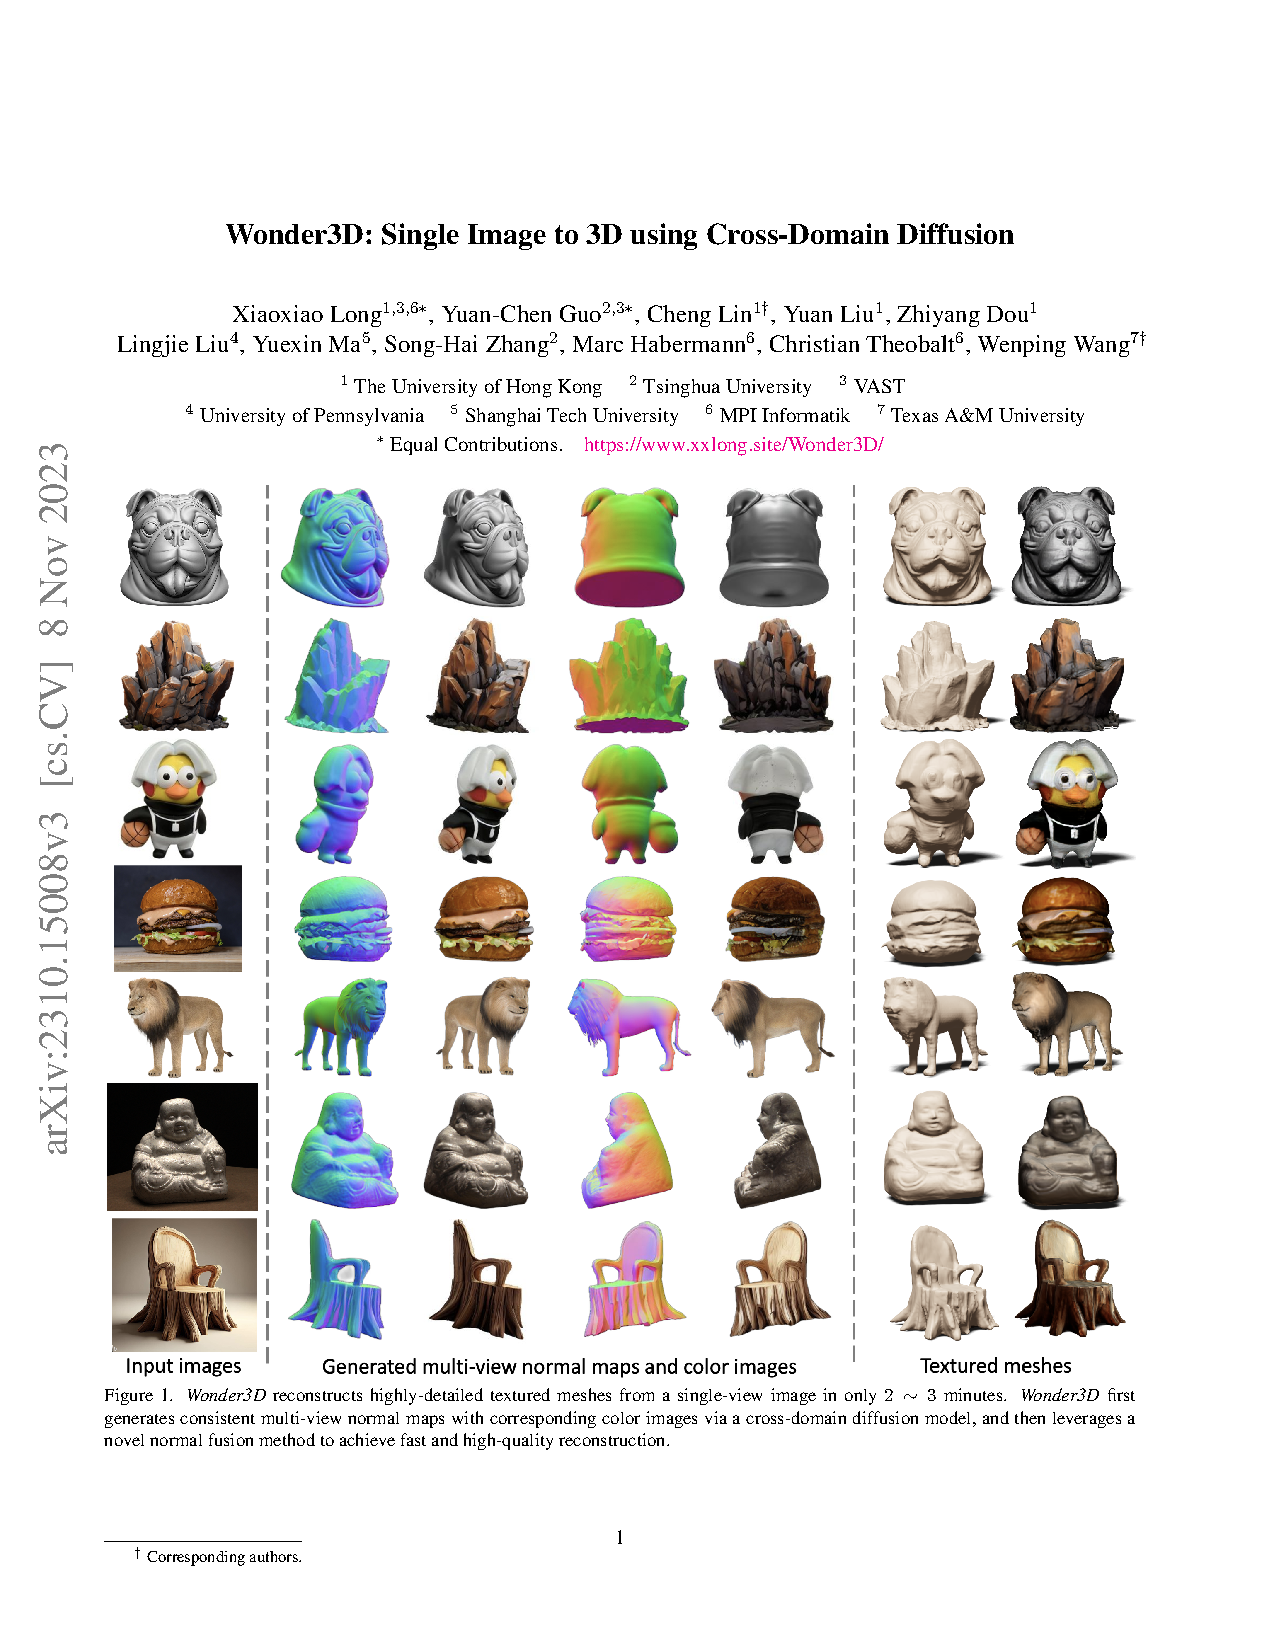
\includegraphics[width=1\columnwidth]{figures/Wonder3D.png}
    \caption{Summarized functionality of Wonder3D, depicting the method's unique approach to generating high-fidelity textured meshes from single images using cross-domain diffusion models \citep{long2023wonder3d}.}\label{fig:Wonder3D}
\end{figure}

The process of generating 3D models from images starts by using CLIP \citep{radfordCLIP} to get a textual description of the image.  

In Wonder3D, the formulation of 3D models is distinctively characterized by modeling the distribution of 3D assets \(p_a{(z)}\) ``as a joint distribution of its corresponding 2D multi-view normal maps and corresponding color images'' \citep{long2023wonder3d}. This modeling allows their training on 2D diffusion models \citep{long2023wonder3d}. The model, conditioned on a given image \( y \), aims to produce multiple normal maps \( n^{1:K} \) and color images \( x^{1:K} \) from various camera perspectives \((\pi_1, \pi_2, \ldots, \pi_k)\), which is achieved by employing a model \( f \), mathematically defined by \citeauthor{long2023wonder3d} as \((n^{1:K}, x^{1:K} | y) = f(y, \pi_{1:k})\).

The creation of the cross-domain joint distribution in Wonder3D is facilitated using a Markov chain within a diffusion framework.~\citeauthor{long2023wonder3d} formally represent this as \[ p\left(n_T^{(1: K)}, x_T^{(1: K)}\right) \prod_t p_\theta\left(n_{t-1}^{(1: K)}, x_{t-1}^{(1: K)} \mid n_t^{(1: K)}, x_t^{(1: K)}\right) \] where \( p\left(n_T^{(1: K)}, x_T^{(1: K)}\right) \) comprises Gaussian noises \citep{long2023wonder3d}.

The model also further enhances its functionality with the generation of consistent multi-view images. This addresses a notable challenge faced by earlier 2D diffusion models, which often produced images with geometric and visual inconsistencies across different views \citep{long2023wonder3d}.

Simply adapting pre-trained stable diffusion models to also output both normal maps and color images, encountered issues with slow convergence and poor generalization \citep{long2023wonder3d}. To address these challenges, Wonder3D introduce a cross-domain diffusion scheme named Domain Switcher \(s\), which is given as an extra input to the diffusion model \citep{long2023wonder3d}. \[
  n^{1:K}, x^{1:K} = f(y, \pi_{1:K}, s_n), f(y, \pi_{1:K}, s_c)
\] This equation by \citeauthor{long2023wonder3d} means that the model uses the switcher \( s \) to determine whether to generate normal maps (\( s_n \)) or color images (\( s_c \)), based on the input provided. However, only using the domain swither does not inherently guarantee geometric consistency between the color image and the normal map for a single view \citep{long2023wonder3d}. To ensure this consistency, Wonder3D employs cross-domain attention, allowing for information exchange between multiple domains, ensuring that the generated normal maps and color images for a particular view are geometrically aligned \citep{long2023wonder3d}.

To transform the 2D normal maps and color images into explicit 3D geometry, Wonder3D optimizes a neural implicit signed distance field (SDF) using a novel optimization scheme. Previous attempts proved challenging due to the sparse nature of the generated views and the subtle inaccuracies in the generated normal maps and color images, leading to distorted geometries, outliers, and incompleteness in the 3D models \citep{long2023wonder3d}.



To overcome these issues, Wonder3D introduces a novel geometric-aware optimization scheme. The optimization process involves segmenting object masks \( M_{0:N} \) from the normal maps \( G_{0:N} \) or color images \( H_{0:N} \) and performing optimization by ``randomly sampling a batch of pixels and their corresponding rays in world space [\(\ldots\)]'' \citep{long2023wonder3d}.

\citeauthor{long2023wonder3d} define the overall objective function as: \[ L = L_{normal} + L_{rgb} + L_{mask} + R_{eik} + R_{sparse} + R_{smooth} \]

The normal loss term, \( L_{normal} \), is key for aligning the 3D geometry with the generated normal maps. It employs a cosine function to maximize the similarity between the normals of the signed distance field (SDF) and the generated normals. The \( L_{rgb} \) term is a mean squared error loss that evaluates the difference between the rendered colors and the generated colors from the model. This term ensures that the color representation in the 3D model closely matches the original images. The \( L_{mask} \) term, a binary cross-entropy loss, calculates the errors between the rendered and generated masks. The eikonal regularization term, \( R_{eik} \), encourages the magnitude of the SDF gradients to maintain unit length, which is important for the stability of the shape's representation. The sparsity regularization term, \( R_{sparse} \), helps avoid isolated, floating parts in the SDF, ensuring a coherent and unified 3D structure. Finally, the smoothness regularization term, \( R_{smooth} \), enforces the smoothness of the SDF gradients in 3D space, contributing to the seamless and natural appearance of the 3D geometry.

